\section{Einleitung}
Das Trägheitsmoment von verschiedenen Körpern soll bestimmt werden und der Satz von Steiner verifiziert werden.
\section{Theorie}
Das Drehmoment $M$, das Trägheitsmoment $I$ als auch die Winkelbeschleunigung $\dot{\omega}$ charakterisieren die Rotationsbewegung.
Für eine punktförmige Masse kann das Trägheitsmoment mit $I = m\cdot r^2$ berechnen. Dabei ist m die Masse und r der Abstand zur Drehachse.
Für ein ausgedehnten Körper um eine feste Achse kann das Gesamtträgheitsmoment dargestellt werden als:

\begin{equation*}
  I=\sum \limits_{i}^{} r_\text{i}^2 \cdot m_\text{i}
\end{equation*}

Das Trägheitsmoment $I$ ist von der Lage der Drehachse abhängig.
Für geometrische Objekte, wie ein Kugel, Stab, Zylinder, lässt sich das Trägheitsmoment
leicht bestimmen.
In Abbildung (\ref{fig:Abb1}) sind verschiedene Objekte mit deren Trägheitsmoment dargestellt.
\begin{figure}[H]
\centering
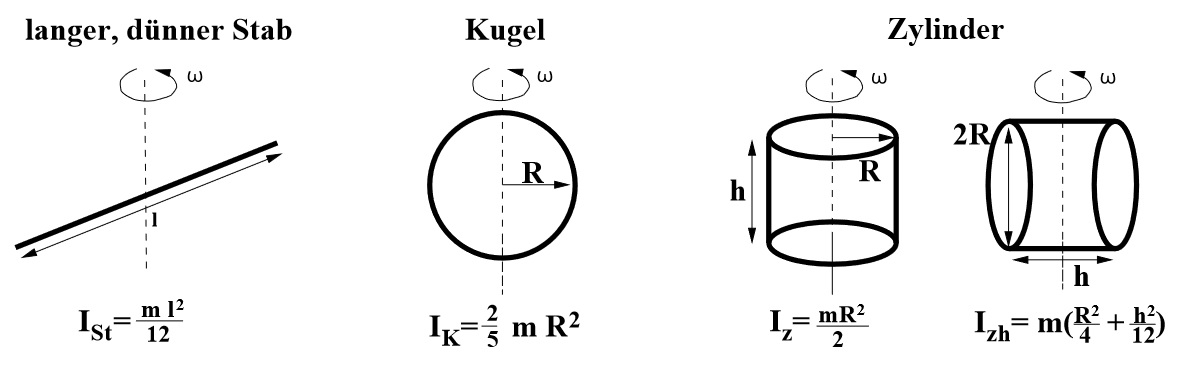
\includegraphics[width=\textwidth]{Bild1.jpg}
\caption{Objekte mit deren Trägheitsmoment[1]}
\label{fig:Abb1}
\end{figure}
Geht die Drehachse nicht durch den Schwerpunkt eines Körpers, sondern parallel um einen Abstand a
zur drehenden Achse verschoben, so lässt sich das Trägheitsmoment mithilfe des Satz von Steiner
\begin{equation}
  I = I_\text{0} + m\cdot a^2
  \label{eq:1}
\end{equation}
erechnen. Dabei ist $I_\text{0}$ das Trägheitsmoment der Drehachse durch den Schwerpunkt des Körpers.
Greift eine Kraft in einem Abstand r von der Achse auf ein drehenden Körper, so wirkt ein Drehmoment $\vec{M} = \vec{F} \times \vec{r}$.
In einem Schwingungssystem wirkt auf einen Körper durch die Drehung um ein Winkel $\phi$ aus seiner Ruhelage ein rücktreibenes Drehmoment
durch eine Feder entgegen. Die harmonische Schwingung lässt sich mit der Schwingungsdauer
\begin{equation}
  T = 2\pi \sqrt{\frac{I}{D}}
  \label{eq:2}
\end{equation}
berechnen. I ist dabei das Trägheitsmoment und D die Winkelrichtsgröße.
\begin{equation}
  D = \frac{M}{\phi} \leftrightarrow D = \frac{F \cdot r}{\phi}
  \label{eq:3}
\end{equation}
Das harmonische Verhalten bei der Drehschwingung ist nur auf kleinen Winekl $\phi$
beschränkt.
